\documentclass[11pt,a4paper]{article}

% ── Packages ──────────────────────────────────────────────────────────────────
\usepackage[margin=2.4cm]{geometry}
\usepackage{graphicx}
\usepackage{booktabs}
\usepackage{tabularx}
\usepackage{longtable}
\usepackage{enumitem}
\usepackage{xcolor}
\usepackage{listings}
\usepackage{hyperref}
\usepackage{fancyhdr}
\usepackage{titlesec}
\usepackage[T1]{fontenc}
\usepackage{lmodern}
\usepackage{microtype}
\usepackage{parskip}

% ── Colours ───────────────────────────────────────────────────────────────────
\definecolor{traigentblue}{HTML}{1A56DB}
\definecolor{codebg}{HTML}{F5F5F5}
\definecolor{keycolor}{HTML}{0550AE}
\definecolor{strcolor}{HTML}{0A3069}
\definecolor{numcolor}{HTML}{953800}
\definecolor{privacygreen}{HTML}{1A7F37}

% ── Listings (JSON) ──────────────────────────────────────────────────────────
\lstdefinelanguage{json}{
  basicstyle=\ttfamily\small,
  backgroundcolor=\color{codebg},
  frame=single,
  rulecolor=\color{black!20},
  framesep=4pt,
  xleftmargin=6pt,
  xrightmargin=6pt,
  breaklines=true,
  showstringspaces=false,
  string=[s]{"}{"},
  stringstyle=\color{strcolor},
  comment=[l]{//},
  commentstyle=\color{black!40}\itshape,
  literate=
    *{:}{{{\color{black}{:}}}}{1}
     {,}{{{\color{black}{,}}}}{1}
     {0}{{{\color{numcolor}{0}}}}{1}
     {1}{{{\color{numcolor}{1}}}}{1}
     {2}{{{\color{numcolor}{2}}}}{1}
     {3}{{{\color{numcolor}{3}}}}{1}
     {4}{{{\color{numcolor}{4}}}}{1}
     {5}{{{\color{numcolor}{5}}}}{1}
     {6}{{{\color{numcolor}{6}}}}{1}
     {7}{{{\color{numcolor}{7}}}}{1}
     {8}{{{\color{numcolor}{8}}}}{1}
     {9}{{{\color{numcolor}{9}}}}{1}
     {true}{{{\color{numcolor}{true}}}}{4}
     {false}{{{\color{numcolor}{false}}}}{5}
     {null}{{{\color{numcolor}{null}}}}{4},
}

% ── Hyperref ──────────────────────────────────────────────────────────────────
\hypersetup{
  colorlinks=true,
  linkcolor=traigentblue,
  urlcolor=traigentblue,
  citecolor=traigentblue,
  pdfauthor={Traigent},
  pdftitle={Hybrid Mode Integration Guide},
}

% ── Headers / footers ────────────────────────────────────────────────────────
\pagestyle{fancy}
\fancyhf{}
\fancyhead[L]{\small\textcolor{black!50}{Traigent --- Hybrid Mode Integration Guide}}
\fancyhead[R]{\small\textcolor{black!50}{Confidential}}
\fancyfoot[C]{\small\thepage}
\renewcommand{\headrulewidth}{0.4pt}

% ── Section styling ──────────────────────────────────────────────────────────
\titleformat{\section}{\Large\bfseries\color{traigentblue}}{}{0em}{}
\titleformat{\subsection}{\large\bfseries}{}{0em}{}
\titleformat{\subsubsection}{\normalsize\bfseries}{}{0em}{}

% ── Macros ────────────────────────────────────────────────────────────────────
\newcommand{\apiendpoint}[2]{\texttt{\textbf{#1}~#2}}
\newcommand{\field}[1]{\texttt{#1}}
\newcommand{\required}{\textbf{Yes}}
\newcommand{\optional}{\textbf{No}}
\newcommand{\status}[1]{\texttt{"#1"}}

% ══════════════════════════════════════════════════════════════════════════════
\begin{document}

% ── Title page ────────────────────────────────────────────────────────────────
\begin{titlepage}
\centering
\vspace*{4cm}
{\Huge\bfseries\color{traigentblue} Hybrid Mode\\[0.3em] Integration Guide\par}
\vspace{1.5cm}
{\Large API Contract \& Optimization Process\par}
\vspace{2cm}
{\large Traigent SDK v1.0\par}
\vspace{0.5cm}
{\large\today\par}
\vspace{3cm}
{\small\textcolor{black!50}{Confidential --- for integration partners only}\par}
\end{titlepage}

\tableofcontents
\clearpage

% ══════════════════════════════════════════════════════════════════════════════
\section{Overview}

Traigent Hybrid Mode enables zero-code optimization of external agentic services.
Your service exposes a lightweight REST API; Traigent's optimizer discovers tunable
parameters, explores configurations, and converges on an optimal setting---all
without accessing your underlying data.

\subsection{What you implement}

A REST service with the prefix \texttt{/traigent/v1/} exposing the endpoints
listed in Section~\ref{sec:endpoints}. Three endpoints are required;
three are optional.

Required endpoints: \texttt{GET /traigent/v1/capabilities},
\texttt{GET /traigent/v1/config-space}, and \texttt{POST /traigent/v1/execute}.

Optional endpoints: \texttt{POST /traigent/v1/evaluate},
\texttt{GET /traigent/v1/health}, and \texttt{POST /traigent/v1/keep-alive}.

\subsection{What Traigent provides}

\begin{itemize}[nosep]
  \item Automatic parameter-space exploration (NSGA-II, Bayesian, grid).
  \item Multi-objective optimization (accuracy, cost, latency, or any custom metric).
  \item Budget controls (max trials, max spend, wall-clock limits).
  \item Statistical promotion via $\varepsilon$-Pareto dominance testing.
\end{itemize}

\subsection{Integration readiness checklist}

Before production rollout, validate that:

\begin{itemize}[nosep]
  \item \texttt{GET /traigent/v1/capabilities} returns \field{version} and accurate feature flags.
  \item \texttt{GET /traigent/v1/config-space} returns a stable \field{capability\_id} and valid \field{tunables}.
  \item \texttt{POST /traigent/v1/execute} enforces capability matching and always returns \field{operational\_metrics.total\_cost\_usd}.
  \item \texttt{POST /traigent/v1/evaluate} is implemented whenever \field{supports\_evaluate=true}.
  \item Optional sections (\field{constraints}, \field{objectives}, \field{exploration}, \field{promotion\_policy}, \field{defaults}, \field{measures}) are omitted unless intentionally used.
\end{itemize}

% ══════════════════════════════════════════════════════════════════════════════
\section{Optimization Process}

The optimization loop follows four phases, repeated until a budget or
convergence criterion is met.

\begin{enumerate}[nosep]
  \item \textbf{Discover} --- Traigent calls \texttt{GET /traigent/v1/capabilities} and
        \texttt{GET /traigent/v1/config-space} to learn which parameters are tunable, their
        domains, and declared objectives.
  \item \textbf{Execute} --- For each trial, Traigent posts a candidate
        configuration and a batch of inputs to \texttt{POST /traigent/v1/execute}. Your
        service runs the agent with those settings and returns per-input
        outputs plus operational metrics (cost, latency, tokens).
  \item \textbf{Evaluate} --- If a separate evaluation endpoint is available,
        Traigent posts output--target pairs to \texttt{POST /traigent/v1/evaluate}. Your
        service scores outputs and returns quality metrics (accuracy,
        relevance, etc.).
  \item \textbf{Optimize} --- Traigent aggregates metrics, updates its
        surrogate model, and selects the next configuration to try. After all
        trials complete, the optimizer ranks configurations by
        $\varepsilon$-Pareto dominance and reports the best.
\end{enumerate}

\begin{figure}[h]
\centering
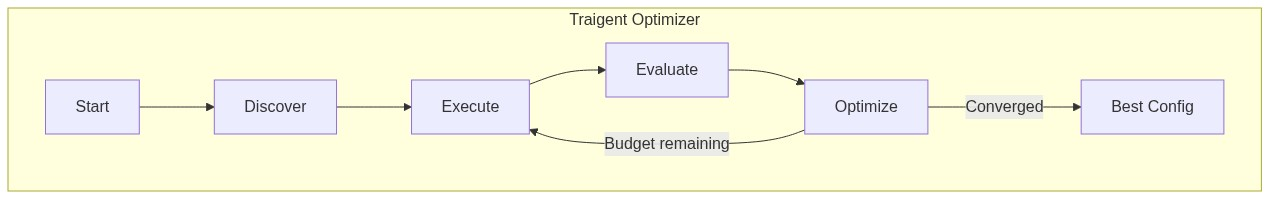
\includegraphics[width=\textwidth]{optimization-loop.jpg}
\caption{Traigent optimization loop: the optimizer iterates through Execute and
Evaluate phases until the budget is exhausted or convergence is reached.}
\label{fig:optimization-loop}
\end{figure}

\begin{center}
\small
\setlength{\tabcolsep}{4pt}
\begin{tabular}{@{}lcl@{}}
\toprule
\textbf{Phase} & \textbf{Direction} & \textbf{Endpoint} \\
\midrule
Discover     & Traigent $\to$ Service & \texttt{GET /traigent/v1/capabilities}, \texttt{GET /traigent/v1/config-space} \\
Execute      & Traigent $\to$ Service & \texttt{POST /traigent/v1/execute} \\
Evaluate     & Traigent $\to$ Service & \texttt{POST /traigent/v1/evaluate} \\
Optimize     & Internal               & (no API call) \\
\bottomrule
\end{tabular}
\end{center}

\subsection{Operational timing guidance}

Use the following targets so clients can set timeout and retry behavior predictably:

\begin{center}\small
\begin{tabularx}{\textwidth}{@{}llX@{}}
\toprule
\textbf{Endpoint} & \textbf{Target latency} & \textbf{Guidance} \\
\midrule
\texttt{GET /traigent/v1/capabilities} & p95 \textless{} 1s & Keep lightweight and cacheable. \\
\texttt{GET /traigent/v1/config-space} & p95 \textless{} 1s & Should be deterministic and idempotent. \\
\texttt{POST /traigent/v1/execute} & p95 \textless{} \field{timeout\_ms} & Default timeout budget is 30s; wrapper returns HTTP 408 when exceeded. \\
\texttt{POST /traigent/v1/evaluate} & p95 \textless{} \field{timeout\_ms} (if provided) & Optional timeout budget; otherwise governed by client transport timeout. \\
\texttt{POST /traigent/v1/keep-alive} & p95 \textless{} 500ms & Heartbeat path should remain fast and side-effect constrained. \\
\bottomrule
\end{tabularx}
\end{center}

\textit{Transport note}: production integrations should use \texttt{HTTPS + HTTP/2}.
Traigent's HTTP client can enforce this in strict mode
(\texttt{create\_transport(..., require\_http2=True)}), which rejects non-HTTPS
endpoints and non-HTTP/2 responses. The v1 contract remains synchronous
request/response. Async job-style APIs and gRPC are future roadmap options, not
part of this contract version.

% ══════════════════════════════════════════════════════════════════════════════
\section{Privacy-Preserving Mode}\label{sec:privacy}

Privacy is the default. Only configuration values and numeric metrics are
observed by Traigent. Input data, output content, and evaluation targets are
\textbf{never} transmitted.

\begin{center}
\small
\begin{tabular}{@{}lc@{}}
\toprule
\textbf{Data} & \textbf{Observed by Traigent} \\
\midrule
Tunable definitions (config-space)             & Yes \\
Configuration values per trial                 & Yes \\
Operational metrics (cost, latency, tokens)    & Yes \\
Quality metrics (accuracy, relevance, etc.)    & Yes \\
Input data content                             & \textcolor{privacygreen}{\textbf{No}} (only IDs) \\
Output data content                            & \textcolor{privacygreen}{\textbf{No}} (only IDs) \\
Target / expected output content               & \textcolor{privacygreen}{\textbf{No}} (only IDs) \\
\bottomrule
\end{tabular}
\end{center}

Your service stores data locally and uses opaque identifiers
(\field{example\_id}, \field{output\_id}, \field{target\_id}) in API exchanges.
If privacy is not a concern, you may include full content in \field{data},
\field{output}, and \field{target} fields. Both modes can be mixed.

% ══════════════════════════════════════════════════════════════════════════════
\section{Authentication (Optional)}

If your service requires authentication, accept a standard
\texttt{Authorization} header (for example a bearer token). Configure the
Traigent optimizer with:

\begin{lstlisting}[basicstyle=\ttfamily\small]
@traigent.optimize(
    execution_mode="hybrid_api",
    hybrid_api_endpoint="https://api.your-service.com",
    tunable_id="my_agent",
    hybrid_api_auth_header="Bearer <token>",
)
\end{lstlisting}

All endpoints must consistently enforce the same authentication policy.
In OpenAPI, this is modelled as optional bearer auth (\texttt{bearerAuth} or anonymous).

\textit{Roadmap}: stronger policy layers (for example RBAC/tenant-scoped roles)
can be added later without changing endpoint shapes.

% ══════════════════════════════════════════════════════════════════════════════
\section{Endpoints}\label{sec:endpoints}

All paths are prefixed with \texttt{/traigent/v1/}.

\subsection{GET /traigent/v1/capabilities \normalfont\textit{(required)}}

Returns service capabilities for the initial handshake.

\subsubsection{Response (200)}

\begin{lstlisting}[language=json]
{
  "version": "1.0",
  "supports_evaluate": true,
  "supports_keep_alive": false,
  "supports_streaming": false,
  "max_batch_size": 100,
  "max_payload_bytes": null,
  "tunable_ids": ["my_agent"]
}
\end{lstlisting}

\textit{Guidance}: omit optional top-level sections when they are not used.
Avoid sending placeholder empty values unless they carry intent.

\begin{center}\small
\begin{tabularx}{\textwidth}{@{}llcX@{}}
\toprule
\textbf{Field} & \textbf{Type} & \textbf{Req.} & \textbf{Description} \\
\midrule
\field{version}              & string  & \required & API version (currently \status{1.0}) \\
\field{supports\_evaluate}   & boolean & \optional & Separate \texttt{/traigent/v1/evaluate} endpoint available (default: \texttt{true}) \\
\field{supports\_keep\_alive}& boolean & \optional & Session heartbeat supported \\
\field{supports\_streaming}  & boolean & \optional & Streaming responses supported \\
\field{max\_batch\_size}     & integer & \optional & Max inputs per execute request (default: 100) \\
\field{max\_payload\_bytes}  & integer & \optional & Max request payload size (\texttt{null}\,=\,unlimited) \\
\field{capability\_ids}      & array[string] & \optional & Optional list of capability IDs supported by this service \\
\bottomrule
\end{tabularx}
\end{center}

\textit{Important}: discovery responses do \textbf{not} return
\field{config\_id} / \field{config\_ids}. The canonical capability identifier
for execution/evaluation is \field{capability\_id} from
\texttt{GET /traigent/v1/config-space}. Per-run identifiers are returned later
by \texttt{POST /traigent/v1/execute} as \field{execution\_id}.

\textit{Note}: \field{capability\_ids} in \texttt{/capabilities} is optional and
primarily useful for service introspection. The canonical capability used for
execution/evaluation is \field{capability\_id} returned by
\texttt{GET /traigent/v1/config-space}.

% ──────────────────────────────────────────────────────────────────────────────
\subsection{GET /traigent/v1/config-space \normalfont\textit{(required)}}

Returns tunable variable definitions. Traigent uses these to build the
parameter search space.

\subsubsection{Response (200)}

\begin{lstlisting}[language=json]
{
  "schema_version": "0.9",
  "tunable_id": "my_agent",
  "tunables": [
    {
      "name": "model",
      "type": "enum",
      "domain": {"values": ["gpt-4o", "claude-3-sonnet", "llama-70b"]},
      "default": "gpt-4o"
    },
    {
      "name": "temperature",
      "type": "float",
      "domain": {"range": [0.0, 2.0], "resolution": 0.1},
      "default": 0.7
    }
  ],
  "objectives": [
    {"name": "accuracy", "direction": "maximize", "weight": 2.0},
    {"name": "cost",     "direction": "minimize", "weight": 1.0}
  ]
}
\end{lstlisting}

\begin{center}\small
\begin{tabularx}{\textwidth}{@{}llcX@{}}
\toprule
\textbf{Field} & \textbf{Type} & \textbf{Req.} & \textbf{Description} \\
\midrule
\field{schema\_version}  & string & \required & TVL schema version (currently \status{0.9}) \\
\field{capability\_id}   & string & \required & Unique identifier for this capability \\
\field{tunables}         & array  & \required & List of tunable definitions (see below) \\
\field{constraints}      & object \textbar{} array & \optional & Structural / behavioral constraints \\
\field{objectives}       & array  & \optional & Objective definitions (name, direction, weight) \\
\field{exploration}      & object & \optional & Strategy, budgets, and convergence criteria \\
\field{promotion\_policy}& object & \optional & $\varepsilon$-Pareto promotion policy \\
\field{defaults}         & object & \optional & Default configuration values \\
\field{measures}         & array  & \optional & Declared metric names produced by the service \\
\bottomrule
\end{tabularx}
\end{center}

\subsubsection{Tunable Definition}

Each element of the \field{tunables} array describes one parameter:

\begin{center}\small
\begin{tabularx}{\textwidth}{@{}llcX@{}}
\toprule
\textbf{Field} & \textbf{Type} & \textbf{Req.} & \textbf{Description} \\
\midrule
\field{name}    & string  & \required      & Variable name (valid Python identifier) \\
\field{type}    & string  & \required      & One of: \texttt{enum}, \texttt{float}, \texttt{int}, \texttt{bool}, \texttt{str} \\
\field{domain}  & object  & Conditional    & Domain specification (required for all types except \texttt{bool}) \\
\field{default} & any     & \optional      & Default value \\
\field{agent}   & string  & \optional      & Agent name for multi-agent grouping \\
\bottomrule
\end{tabularx}
\end{center}

\subsubsection{Tunable Types}

\begin{center}\small
\begin{tabularx}{\textwidth}{@{}llX@{}}
\toprule
\textbf{Type} & \textbf{Domain format} & \textbf{Example} \\
\midrule
\texttt{enum}  & \texttt{\{"values": [...]\}} & \texttt{["gpt-4o", "claude-3-sonnet"]} \\
\texttt{float} & \texttt{\{"range": [min, max], "resolution": step\}} & \texttt{[0.0, 2.0]}, step 0.1 \\
\texttt{int}   & \texttt{\{"range": [min, max]\}} & \texttt{[100, 4096]} \\
\texttt{bool}  & N/A & \texttt{true} / \texttt{false} \\
\texttt{str}   & \texttt{\{"values": [...]\}} & \texttt{["concise", "detailed"]} \\
\bottomrule
\end{tabularx}
\end{center}

% ──────────────────────────────────────────────────────────────────────────────
\subsection{POST /traigent/v1/execute \normalfont\textit{(required)}}\label{sec:execute}

Execute the agent with a specific configuration on a batch of inputs.

\subsubsection{Request}

\begin{lstlisting}[language=json]
{
  "request_id": "550e8400-e29b-41d4-a716-446655440000",
  "tunable_id": "my_agent",
  "config": {
    "model": "gpt-4o",
    "temperature": 0.5,
    "max_tokens": 1024
  },
  "examples": [
    {"example_id": "ex_001", "data": {"query": "What is machine learning?"}},
    {"example_id": "ex_002", "data": {"query": "Explain neural networks"}}
  ],
  "timeout_ms": 30000
}
\end{lstlisting}

\begin{center}\small
\begin{tabularx}{\textwidth}{@{}llcX@{}}
\toprule
\textbf{Field} & \textbf{Type} & \textbf{Req.} & \textbf{Description} \\
\midrule
\field{request\_id}    & string (UUID) & \optional & Idempotency key (auto-generated if omitted) \\
\field{capability\_id} & string        & \required & Capability to invoke \\
\field{config}         & object        & \required & Configuration parameters (tunable values) \\
\field{examples}       & array         & \required & Examples to process \\
\field{session\_id}    & string        & \optional & Session ID for stateful agents \\
\field{batch\_options} & object        & \optional & Parallelism, fail-fast, per-item timeout \\
\field{timeout\_ms}    & integer       & \optional & Request timeout in ms (default: 30\,000) \\
\bottomrule
\end{tabularx}
\end{center}

Each \textbf{Input Item} contains:

\begin{center}\small
\begin{tabularx}{\textwidth}{@{}llcX@{}}
\toprule
\field{example\_id} & string & \required & Unique identifier for this input \\
\field{data}      & object & \optional & Input data (omit in privacy-preserving mode) \\
\bottomrule
\end{tabularx}
\end{center}

\subsubsection{Response (200)}

\begin{lstlisting}[language=json]
{
  "request_id": "550e8400-e29b-41d4-a716-446655440000",
  "execution_id": "exec_123456",
  "status": "completed",
  "outputs": [
    {
      "example_id": "ex_001",
      "output": {"response": "Machine learning is a subset of AI..."},
      "cost_usd": 0.002,
      "latency_ms": 150
    }
  ],
  "operational_metrics": {
    "total_cost_usd": 0.005,
    "latency_ms": 330,
    "tokens_used": 450
  }
}
\end{lstlisting}

\begin{center}\small
\begin{tabularx}{\textwidth}{@{}llcX@{}}
\toprule
\textbf{Field} & \textbf{Type} & \textbf{Req.} & \textbf{Description} \\
\midrule
\field{request\_id}          & string & \required & Echoed request ID for correlation \\
\field{execution\_id}        & string & \required & Unique execution ID (referenced by \texttt{/traigent/v1/evaluate}) \\
\field{status}               & string & \required & \status{completed}, \status{partial}, or \status{failed} \\
\field{outputs}              & array  & \required & Per-input results (see Output Item below) \\
\field{operational\_metrics} & object & \required & Aggregate operational metrics \\
\field{quality\_metrics}     & object & \optional & Quality metrics (combined execute+evaluate mode) \\
\field{session\_id}          & string & \optional & Session ID for stateful agents \\
\field{error}                & object & \optional & Error details if \field{status} is \status{failed} or \status{partial} \\
\bottomrule
\end{tabularx}
\end{center}

Each \textbf{Output Item} contains:

\begin{center}\small
\begin{tabularx}{\textwidth}{@{}llcX@{}}
\toprule
\field{example\_id}   & string & \required & Matching input identifier \\
\field{output}      & object & \optional & Agent output (omit in privacy-preserving mode) \\
\field{output\_id}  & string & \optional & Output identifier (privacy-preserving mode) \\
\field{cost\_usd}   & number & \optional & Cost for this input \\
\field{latency\_ms} & number & \optional & Latency for this input \\
\field{metrics}     & object & \optional & Per-input quality metrics (combined mode) \\
\field{error}       & string & \optional & Error message for partial failures \\
\bottomrule
\end{tabularx}
\end{center}

\subsubsection{Operational Metrics}

\field{total\_cost\_usd} is the only required field. Additional recommended and custom
metrics may be included:

\begin{center}\small
\begin{tabularx}{\textwidth}{@{}llX@{}}
\toprule
\textbf{Field} & \textbf{Type} & \textbf{Description} \\
\midrule
\field{total\_cost\_usd} & number  & \textbf{Required.} Total cost in USD \\
\field{latency\_ms}      & number  & Recommended. Total latency in milliseconds \\
\field{tokens\_input}    & integer & Input token count \\
\field{tokens\_output}   & integer & Output token count \\
\field{cache\_hit\_rate}  & number  & Cache hit ratio (0.0--1.0) \\
\field{retry\_count}     & integer & Number of retries \\
\multicolumn{3}{@{}l}{\itshape Any additional numeric, string, or boolean fields are accepted.} \\
\bottomrule
\end{tabularx}
\end{center}

% ──────────────────────────────────────────────────────────────────────────────
\subsection{POST /traigent/v1/evaluate \normalfont\textit{(optional)}}\label{sec:evaluate}

Evaluate outputs against expected targets. Only required when
\field{supports\_evaluate} is \texttt{true} in capabilities.

\subsubsection{Request}

\begin{lstlisting}[language=json]
{
  "request_id": "660e8400-e29b-41d4-a716-446655440001",
  "tunable_id": "my_agent",
  "execution_id": "exec_123456",
  "evaluations": [
    {
      "example_id": "ex_001",
      "output": {"response": "Machine learning is a subset of AI..."},
      "target": {"expected": "Machine learning is a branch of AI..."}
    }
  ],
  "timeout_ms": 30000
}
\end{lstlisting}

\begin{center}\small
\begin{tabularx}{\textwidth}{@{}llcX@{}}
\toprule
\textbf{Field} & \textbf{Type} & \textbf{Req.} & \textbf{Description} \\
\midrule
\field{request\_id}    & string (UUID) & \optional & Idempotency key \\
\field{capability\_id} & string        & \required & Evaluation capability identifier \\
\field{execution\_id}  & string        & \optional & Reference to previous execute \\
\field{evaluations}    & array         & \optional & Output--target pairs (typically non-empty) \\
\field{config}         & object        & \optional & Evaluation parameters \\
\field{session\_id}    & string        & \optional & Session ID for stateful agents \\
\field{timeout\_ms}    & integer       & \optional & Optional timeout budget in ms (wrapper emits 408 on timeout) \\
\bottomrule
\end{tabularx}
\end{center}

\textit{Note}: \field{capability\_id} is validated against the configured service capability.

Each \textbf{Evaluation Item} contains:

\begin{center}\small
\begin{tabularx}{\textwidth}{@{}llcX@{}}
\toprule
\field{example\_id}   & string & \required & Matching input identifier \\
\field{output}      & object & \optional & Agent output (or use \field{output\_id}) \\
\field{output\_id}  & string & \optional & Output reference (privacy-preserving mode) \\
\field{target}      & object & \optional & Expected output (or use \field{target\_id}) \\
\field{target\_id}  & string & \optional & Target reference (privacy-preserving mode) \\
\bottomrule
\end{tabularx}
\end{center}

\subsubsection{Response (200)}

\begin{lstlisting}[language=json]
{
  "request_id": "660e8400-e29b-41d4-a716-446655440001",
  "status": "completed",
  "results": [
    {
      "example_id": "ex_001",
      "metrics": {"accuracy": 0.92, "relevance": 0.88, "fluency": 0.95}
    }
  ],
  "aggregate_metrics": {
    "accuracy":  {"mean": 0.92, "std": 0.05, "n": 100},
    "relevance": {"mean": 0.88, "std": 0.03, "n": 100}
  }
}
\end{lstlisting}

\begin{center}\small
\begin{tabularx}{\textwidth}{@{}llcX@{}}
\toprule
\textbf{Field} & \textbf{Type} & \textbf{Req.} & \textbf{Description} \\
\midrule
\field{request\_id}        & string & \required & Echoed request ID \\
\field{status}             & string & \required & \status{completed}, \status{partial}, or \status{failed} \\
\field{results}            & array  & \required & Per-example evaluation results \\
\field{aggregate\_metrics} & object & \required & Aggregated statistics per metric \\
\field{error}              & object & \optional & Error details for partial/failed evaluations \\
\bottomrule
\end{tabularx}
\end{center}

Each \textbf{Result Item}: \field{example\_id}~(required), \field{metrics}~(required object of numeric quality scores), \field{error}~(optional string).

Each \textbf{Aggregate Metric}: \field{mean}~(number), \field{std}~(number), \field{n}~(integer).

% ──────────────────────────────────────────────────────────────────────────────
\subsection{GET /traigent/v1/health \normalfont\textit{(optional)}}

Health check for monitoring and load-balancer probes.

\begin{center}\small
\begin{tabularx}{\textwidth}{@{}llcX@{}}
\toprule
\textbf{Field} & \textbf{Type} & \textbf{Req.} & \textbf{Description} \\
\midrule
\field{status}          & string & \required & \status{healthy}, \status{degraded}, or \status{unhealthy} \\
\field{version}         & string & \optional & Service version \\
\field{uptime\_seconds} & number & \optional & Uptime in seconds \\
\field{details}         & object & \optional & Additional health details \\
\bottomrule
\end{tabularx}
\end{center}

% ──────────────────────────────────────────────────────────────────────────────
\subsection{POST /traigent/v1/keep-alive \normalfont\textit{(optional)}}

Session heartbeat for stateful agents.
Only implement if \field{supports\_keep\_alive} is \texttt{true} in capabilities.

\textbf{Request}: \texttt{\{"session\_id": "session\_abc123"\}}

\textbf{200 Response}: \texttt{\{"status": "alive", "session\_id": "session\_abc123"\}}

\textbf{404 Response}: \texttt{\{"error": \{"code": "SESSION\_NOT\_FOUND", "message": "..."\}\}}

% ══════════════════════════════════════════════════════════════════════════════
\section{Error Responses}

All endpoints must return structured errors with appropriate HTTP status codes.

\begin{center}\small
\begin{tabularx}{\textwidth}{@{}clX@{}}
\toprule
\textbf{Status} & \textbf{Description} & \textbf{Client behavior} \\
\midrule
400 & Bad Request (invalid input, capability mismatch) & Do not retry until payload is fixed. \\
401 & Unauthorized (when endpoint authentication is enabled) & Refresh/reconfigure credentials, then retry. \\
404 & Not Found (unknown route or session) & Re-discover endpoint/state before retry. \\
408 & Request Timeout (\field{timeout\_ms} exceeded) & Retry with backoff and/or larger timeout budget. \\
429 & Too Many Requests (rate limited) & Retry with backoff; respect \texttt{Retry-After}. \\
500 & Internal Server Error & Retry with bounded backoff and alert if persistent. \\
503 & Service Unavailable & Retry with backoff; respect \texttt{Retry-After}. \\
\bottomrule
\end{tabularx}
\end{center}

\textit{Note}: endpoint-specific response sets are defined in
\texttt{hybrid-mode-openapi.yaml} and are the normative source.

Error body format:

\begin{lstlisting}[language=json]
{
  "error": {
    "code": "INVALID_CONFIG",
    "message": "Unknown tunable: invalid_param",
    "details": {"invalid_params": ["invalid_param"]}
  }
}
\end{lstlisting}

\subsection{Observability and trace context}

For distributed tracing, clients may send W3C headers:
\texttt{traceparent} and \texttt{tracestate}. Wrapper responses echo these
headers and include \texttt{x-traigent-request-id} when a request/response
contains \field{request\_id}. Keep \field{request\_id} for business-level
correlation and trace headers for span-level correlation.

% ══════════════════════════════════════════════════════════════════════════════
\section{Idempotency}

\texttt{GET /traigent/v1/capabilities}, \texttt{GET /traigent/v1/config-space}, and
\texttt{GET /traigent/v1/health} should be side-effect free and idempotent by contract.

\texttt{POST /traigent/v1/execute} and \texttt{POST /traigent/v1/evaluate} accept \field{request\_id}
(UUID recommended). If the same \field{request\_id} is received again, the
service may return a cached response. This enables safe retries without
duplicate processing.

Required server behavior for idempotency keys:
\begin{itemize}[nosep]
  \item Same \field{request\_id} + same payload $\rightarrow$ return cached response.
  \item Same \field{request\_id} + different payload $\rightarrow$ return HTTP 400.
\end{itemize}

The \texttt{POST /traigent/v1/keep-alive} endpoint uses \field{session\_id} and does not
require \field{request\_id}.

\textit{Wrapper note}: \texttt{TraigentService} implements in-process idempotency
for \texttt{/execute} and \texttt{/evaluate}. If custom servers do not implement
idempotency, retrying the same request can execute work twice and duplicate
side effects/cost.

\textit{Optional extension}: \texttt{OPTIONS} can be implemented for method
discovery/CORS convenience, but is not required by the core hybrid contract.

% ══════════════════════════════════════════════════════════════════════════════
\section{Accompanying Specifications}

The following machine-readable files are provided alongside this document and
constitute the normative contract:

\begin{center}\small
\begin{tabularx}{\textwidth}{@{}llX@{}}
\toprule
\textbf{File} & \textbf{Format} & \textbf{Usage} \\
\midrule
\texttt{hybrid-mode-openapi.yaml}   & OpenAPI 3.0.3 & Client/server codegen, request/response validation, Swagger UI \\
\texttt{hybrid-mode-schemas.json}   & JSON Schema (Draft 2020-12) & Standalone DTO validation \\
\texttt{hybrid-mode-api-contract.md}& Markdown & Full endpoint reference with examples \\
\texttt{hybrid-mode-client-guide.md}& Markdown & Implementation patterns, code samples, troubleshooting \\
\bottomrule
\end{tabularx}
\end{center}

\subsection{Generating client stubs}

\begin{lstlisting}[language=json,basicstyle=\ttfamily\footnotesize]
// Python
openapi-generator generate -i hybrid-mode-openapi.yaml -g python -o client/

// TypeScript
openapi-generator generate -i hybrid-mode-openapi.yaml -g typescript-fetch -o client/
\end{lstlisting}

\subsection{Validation and linting}

\begin{lstlisting}[basicstyle=\ttfamily\footnotesize]
# Validate syntax and references
npx @apidevtools/swagger-cli validate hybrid-mode-openapi.yaml

# Lint for OpenAPI best practices
npx @redocly/cli lint hybrid-mode-openapi.yaml
\end{lstlisting}

\subsection{Publish as single source of truth}

Publish \texttt{hybrid-mode-openapi.yaml} in Swagger UI/Redoc from versioned git
tags (for example \texttt{v1.0.0}, \texttt{v1.0.1}). Avoid distributing
hand-edited zip snapshots as the primary contract source.

% ══════════════════════════════════════════════════════════════════════════════
\section{Quick Reference}

\begin{center}\small
\begin{tabularx}{\textwidth}{@{}lllX@{}}
\toprule
\textbf{Method} & \textbf{Path} & \textbf{Req.} & \textbf{Purpose} \\
\midrule
\texttt{GET}  & \texttt{/traigent/v1/capabilities} & \required & Service handshake \\
\texttt{GET}  & \texttt{/traigent/v1/config-space}  & \required & Tunable definitions \\
\texttt{POST} & \texttt{/traigent/v1/execute}       & \required & Run agent with config \\
\texttt{POST} & \texttt{/traigent/v1/evaluate}      & \optional & Score outputs vs.\ targets \\
\texttt{GET}  & \texttt{/traigent/v1/health}        & \optional & Health check \\
\texttt{POST} & \texttt{/traigent/v1/keep-alive}    & \optional & Session heartbeat \\
\bottomrule
\end{tabularx}
\end{center}

\end{document}
